\documentclass[../defence.tex]{subfiles}
\begin{document}
  \begin{frame}{Barrier layer thickness - nonisotrope etch rate}
    \begin{columns}[onlytextwidth, T]
      \column{\dimexpr\linewidth / 21 * 10}
        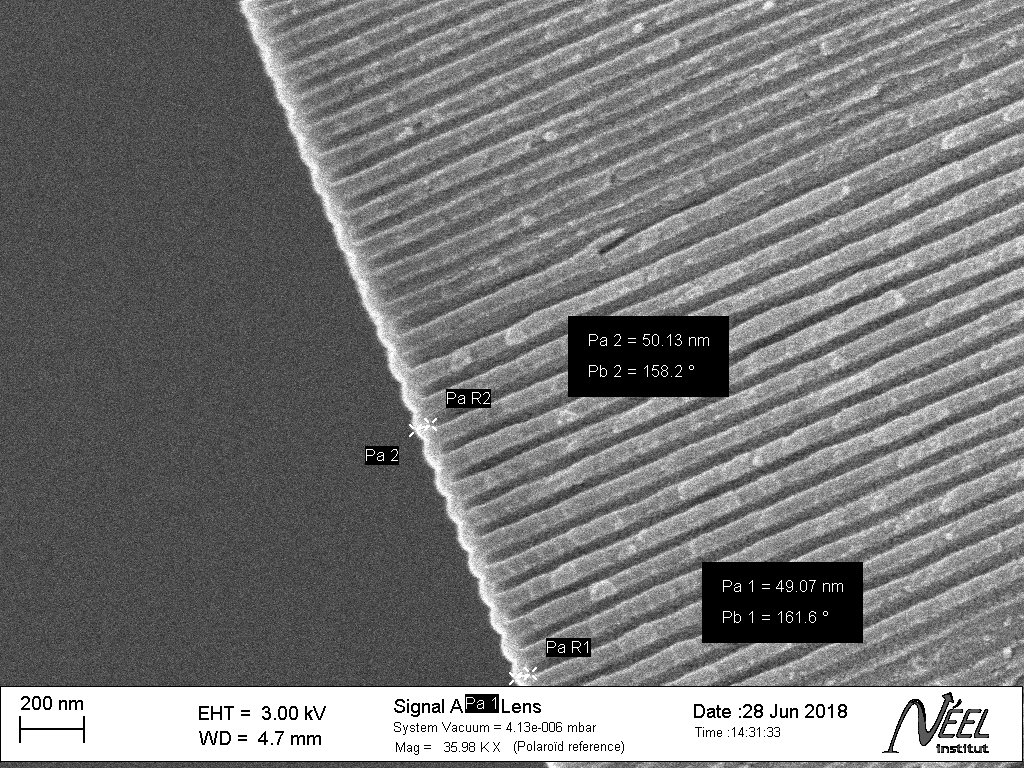
\includegraphics[width=\linewidth]{images/296c_barrier_layer.jpg}
        \pause

        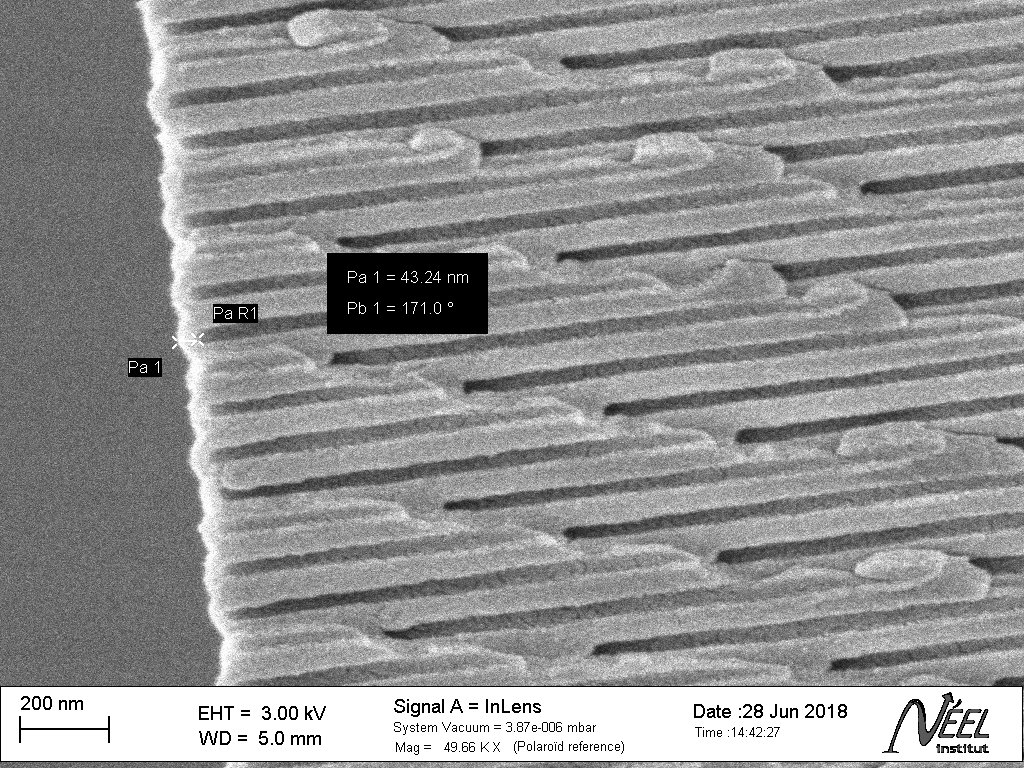
\includegraphics[width=\linewidth]{images/296e_barrier_layer_meb.jpg}
        \pause

    \column{\dimexpr\linewidth / 21}
    \column{\dimexpr\linewidth / 21 * 10}
      \begin{alertbox}{Barrier layer thickness}
        \begin{tiny}
          \begin{itemize}
            \item Assumed to always be $\SI{30}{\nano\meter}$
            \pause

            \item Has not been probed before the treatments
            \pause

            \item Much too large \textsc{after} floating
            \pause

            \item Not uniform over multiple wafers; uniformity on a given wafer remains to be probed
            \pause

            \item Etch rate much stronger than within the pores
          \end{itemize}
        \end{tiny}
      \end{alertbox}
    \end{columns}
  \end{frame}
\end{document}
